\documentclass{article}

\usepackage{mathrsfs,amsmath}
\usepackage{xcolor}
\usepackage{titlesec}
\usepackage{listings}
\usepackage{syntax}
\usepackage{pythonhighlighting}
\usepackage{graphicx}

\usepackage[margin=1.4in]{geometry}
\graphicspath{ {./images/} }

\title{Exercise \#00 | CS 335} 
\author{Jared Dyreson\\ 
        California State University, Fullerton}

\DeclareRobustCommand{\bowtie}{%
  \mathrel\triangleright\joinrel\mathrel\triangleleft}


\usepackage [english]{babel}
\usepackage [autostyle, english = american]{csquotes}
\MakeOuterQuote{"}

\titlespacing*{\section}
{0pt}{5.5ex plus 1ex minus .2ex}{4.3ex plus .2ex}
\titlespacing*{\subsection}
{0pt}{5.5ex plus 1ex minus .2ex}{4.3ex plus .2ex}

\usepackage{hyperref}
\hypersetup{
    colorlinks,
    citecolor=black,
    filecolor=black,
    linkcolor=black,
    urlcolor=black
}

\begin{document}

\maketitle
\tableofcontents

\newpage

\section{Examples}

\subsection{Arithmetic}

\begin{flushleft}

\textbf{Problem:}

\begin{python}
def arithmetic(lst):
    x = lst[0]
    y = lst[1]
    lst[2] = x + y
    return lst[0] + lst[1]
\end{python}

\textbf{Analysis:} Each line only contains one 1 step, therefore it linear. Thus having a classification of $O(n)$.

\end{flushleft}

\subsection{Nested Function Calls}

\begin{flushleft}

\begin{python}
def setup():
    forward = make_list(20) # n + 3 : dependent of defined size and contents of function called below
    backward = make_list(30) # n + 3 ^ see above
    return forward, backward # 1
    # 2(n + 3) + 1 => 2n + 6 + 1 => 2n + 7

def make_list(n):
    L = [] # 1
    for i in range(n): # n
        L.append(0) # 1
    return L # 1
    # 1 + n + 1  + 1 => n + 3
\end{python}

\textbf{Analysis:} Therefore, the current runtime is $O(2n + 7)$. However, since we are classifying algorithms in Big Oh, we ignore leading coefficients and only focus on the leading term.
Thus, the true classification of this algorithm is of $O(n)$, as it is directly proportional to the input of the problem set.

\end{flushleft}

\subsection{Loops}

$$T(n) = \sum_{x \in X} t_{x}$$

\begin{flushleft}

\begin{python}
for x in range(100):
    print("hello") # please assume printing only takes one instruction/atomic
    print("world")
    print("goodbye")
\end{python}

\textbf{Analysis:} Since this loop only contains atomics, we can add up the amount of them and use it as our coefficient. Thus becoming: $O(3n) \implies O(n)$

\end{flushleft}

\subsection{Loops in Sequence}

\begin{flushleft}
\begin{python}
def func():
    for x in range(100):
        # contains three atomics
        print("hello")
        print("hello")
        print("hello")
    for x in range(1000):
        # contains two atomics
        print("world")
        print("hello")
\end{python}

\textbf{Analysis:} Since both of these loops only contain atomics, we can add up the amount of them and use it as our coefficient for each. Both loops are independent of one another and do not contribute to the overall runtime classification. Thus becoming: $( O(3n) + O(2n) ) \implies O(5n) \implies O(n)$

\end{flushleft}


\subsection{Nested Loops}

\begin{flushleft}

\begin{python}
for x in range(10):
    # three atomics
    for y in range(10):
        # two atomics
\end{python}

\textbf{Analysis:} When attempting to analyze the runtime of nested loops, we need to count how many loop calls there are. This will give us the degree our polynomial will be. These instructions compound on one another, as the parent must execute along with all it's children. In this case, our deepest for loop call is of $O(2n)$ and our parent is $O(3n)$. We can determine the runtime by saying that:

$$O(2n) \times O(3n) \implies O(6n^{2}) \implies O(n^{2})$$

\end{flushleft}

\newpage

\section{General Notes}

\begin{itemize}
\item If a math function gives a large resultant from a small input size, please refrain from using this algorithm

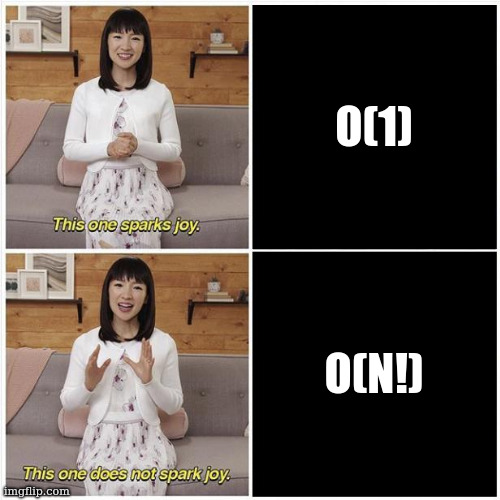
\includegraphics[width=7cm]{joy.jpg}
\end{itemize}

\end{document}

